\section{Subsistema: Estrutura} \label{sec:estrutura}

As dimensões do carrinho foram feitas com base na ergonomia utilizando uma cadeira de rodas como base. A altura máxima do carrinho será de 800mm para que o cadeirante tenha facilidade de colocar e retirar os objetos nele.

\par As dimensões da cesta foram de 800mm de comprimento, 500mm de largura e 250mm de profundidade. Os 500mm de largura levou em consideração a largura da cadeira de rodas. Essa largura permite que o carrinho esteja atrás do cadeirante sem que ocupe um espaço maior que o da cadeira no corredor. O comprimento e a profundidade foram com base no volume de 100L que o carrinho será capaz de transportar e levando em consideração a capacidade do cadeirante de retirar objetos sem dificuldades.

\par Na base do carrinho será uma chapa de alumínio onde serão fixados os motores, as rodas e as baterias, sendo necessário a fabricação de suportes. Ele possuirá quatro suportes que irão unir a base e a cesta do carrinho.

%2 imagens
 \begin{figure}[ht]
		\centering
		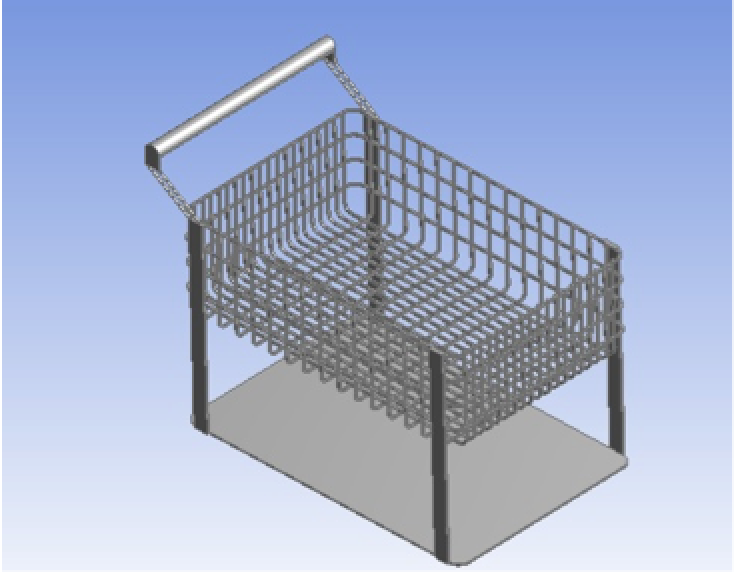
\includegraphics[width=.4\textwidth]{figuras/CADcarrinho.png}
		\caption{CAD da estrutura do carrinho}
		\label{fig:CADcarrinho}
	\end{figure} 
    
 \begin{figure}[ht]
		\centering
		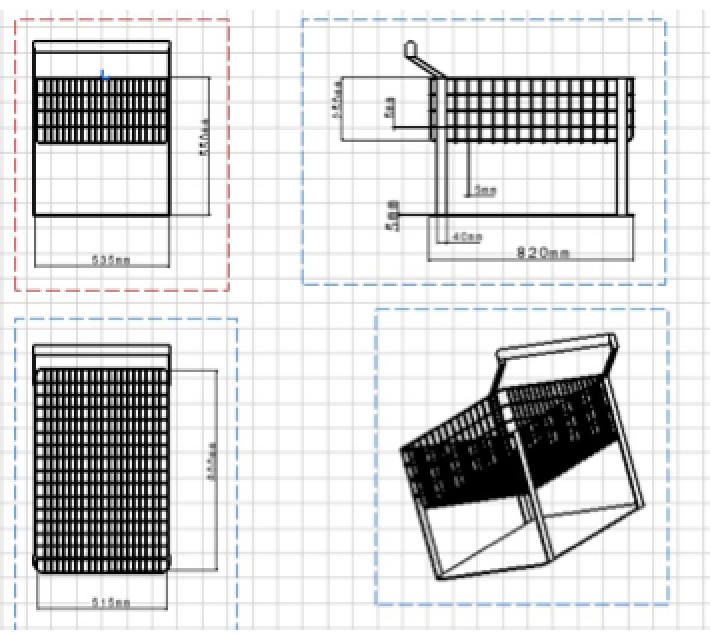
\includegraphics[width=.4\textwidth]{figuras/estrutura.png}
		\caption{Dimensões da estrutura do carrinho}
		\label{fig:estrutura}
	\end{figure} 

\subsection{Material}

\par Foi escolhido o alumínio para ser usado na estrutura, pois o carrinho estará em uso constante nos supermercados, comportando um peso considerável e sofrendo vibração devido ao atrito com o piso conforme onde este é usado. Qualquer ação diária faz com que o carrinho sofra desgastes e se o material for frágil ele se danificará facilmente.

\par O alumínio é leve e resistente, pesando 1/3 do peso do aço, possuindo densidade de $2.7\frac{g}{cm^3}$ . O peso baixo do alumínio é uma vantagem para a aplicação no carrinho, pois diminui o peso total do carrinho, diminuindo assim a força necessária para movimentar o carrinho. Outra vantagem consiste em ele ser altamente resistente a corrosão, pois possui uma camada protetora de óxido.

\subsection{Rodas}
O ideal é que o equipamento disponha de rodas de aço e giratórias, que deslizam com facilidade, independente do tipo de piso, funcionando bem tanto para um piso liso, como o do mercado, como para um piso com rugosidade, semelhante ao estacionamento do supermercado, precisando assim de uma rodinha que não danifique facilmente.

\par As rodas traseiras e dianteiras serão com rodízio, tendo diâmetro de 101 mm e largura de 27mm de largura, resistindo um peso 60kg por rodinha.

\subsection{Transmissão}

O uso da transmissão irá depender do motor utilizado no projeto, caso o motor não possua torque necessário para movimentar o carrinho, será necessário uma transmissão para aumentar o torque que entra na roda traseira do carrinho.
	
\par Existem diversos tipos de elementos que são utilizados para fazer a transmissão da potência do motor para as rodas, como por exemplo as correias, as correntes e as engrenagens. Em alguns casos, elas simplificam o projeto, reduzindo assim o custo \cite{Projmec}.

\subsection{Correias}
Existem quatro tipos de correias: as correias planas, que utilizam polias coroadas; correias redondas, que utilizam polias ranhuradas ou acanaladas; correias em V, que utilizam os mesmos tipos de polias das correias redondas; correias de tempo, que utilizam rodas dentadas, ou catracas.
	
\par Os eixos precisam ser separados por uma distância mínima, dependendo da correia e do seu tamanho, para que assim esta possa trabalhar apropriadamente. As correias podem ser utilizadas para longas distâncias de centro.


\subsection{Engrenagens}
As forças transmitidas pelas engrenagens quando estas estão engrazadas geram momentos torcionais, gerando movimento e a transmissão da potência.

\par Para que ser transmitida essa potência, é necessário que as engrenagens tenham uma ação conjugada, onde a razão entre as velocidades angulares deve ser constante

\par Existem diversas maneiras para se fabricar dentes de engrenagens, como por exemplo a fundição em areia, fundição de investimento, fundição em molde permanente, moldagem em casa, entre outros \cite{Projmaq}.
\par Dentre os modelos de transmissão, foi selecionado inicialmente a correia plana, por ser mais silenciosa, por sua eficiência de 98\% e pela sua praticidade no ajuste de seu comprimento. Porém, ... optou-se por correia em V pois ...








	



























